\newcommand{\makeNAMEFig}{%
\begin{figure}[tbp]
    \centering
    \includegraphics[width=\linewidth]{figures/NAME}
    \caption{CAPTION}
    \label{fig:NAME}
\end{figure}
}

\newcommand{\makeSampleSegFig}{%
\begin{figure}[tbp]
    \centering
    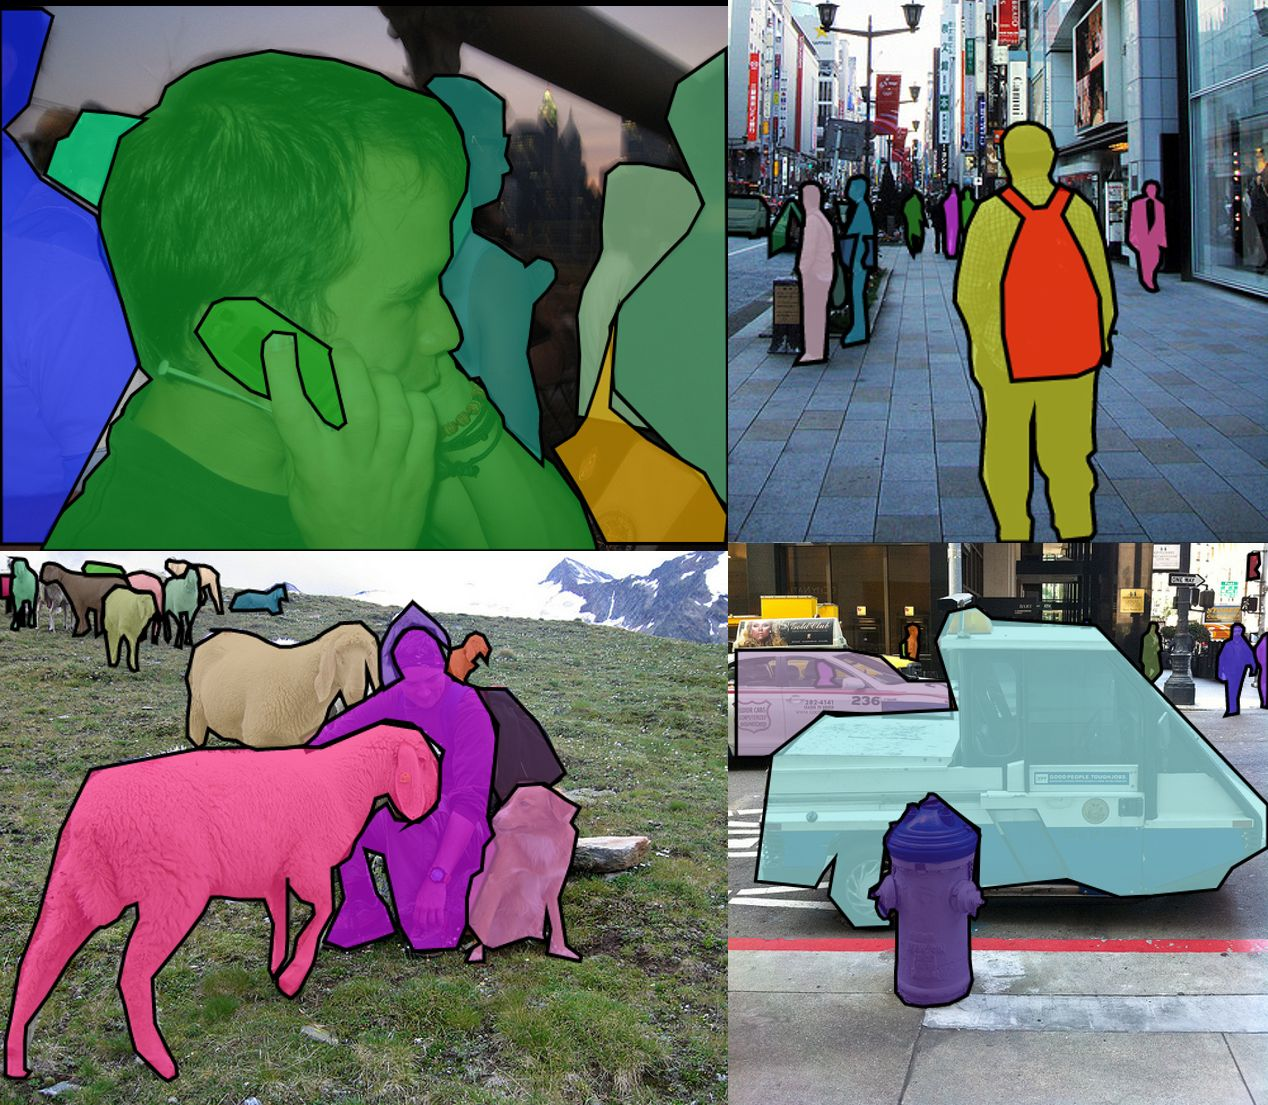
\includegraphics[width=0.75\linewidth]{figures/sampleSegData}
    \caption{Common use cases for semantic segmentation involve relatively few foreground objects, low-resolution data, and limited complexity per object. Images retrieved from \url{https://cocodataset.org/\#explore}.}
    \label{fig:sampleSegData}
\end{figure}
}

\newcommand{\makePcbFig}{%
\begin{figure}[tbp]
    \centering
    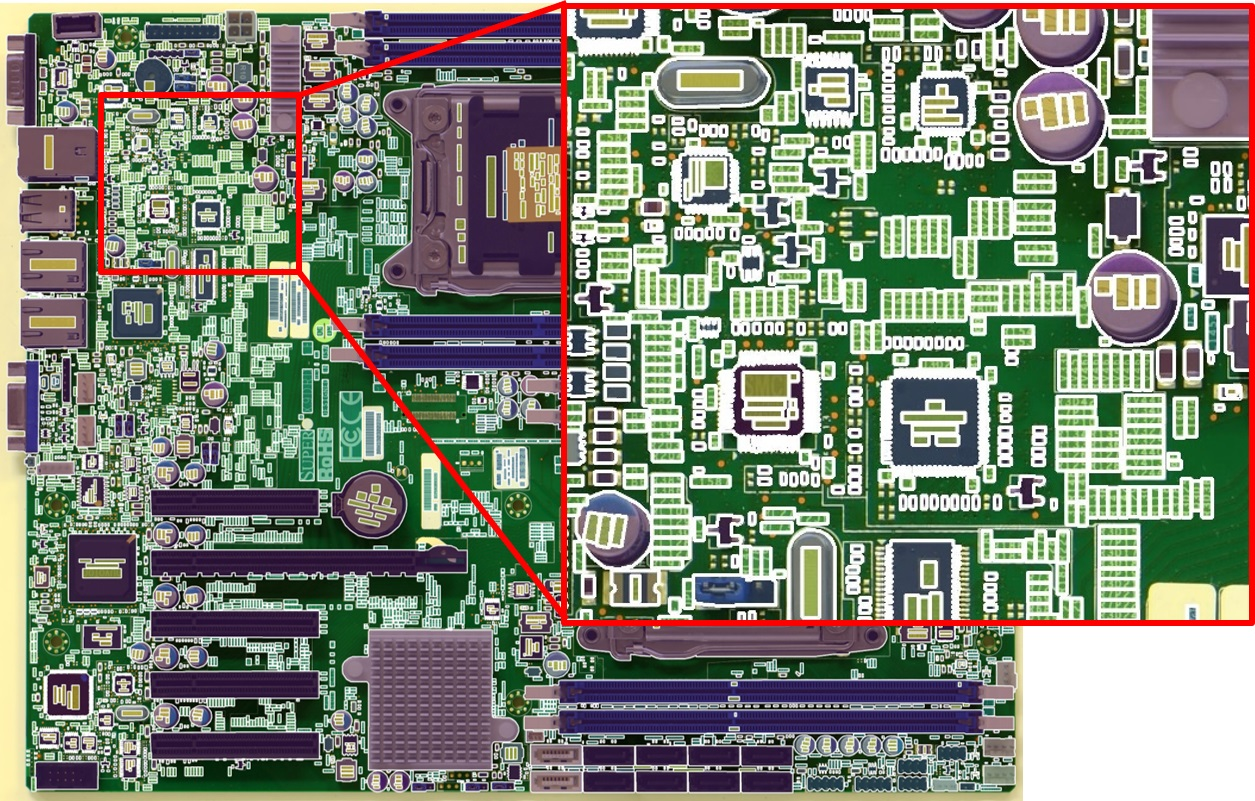
\includegraphics[width=\linewidth]{figures/pcb}
    \caption{Example PCB segmentation. In contrast to typical semgentation tasks, the scene contains over 4,000 objects with numerous complex shapes.}
    \label{fig:pcb}
\end{figure}
}


\newcommand{\makeFeedbackLoopFig}{%
\begin{figure}[tbp]
	\centering
	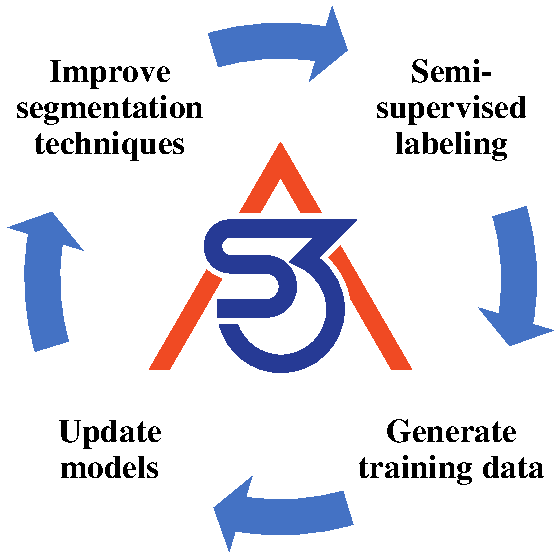
\includegraphics[width=0.5\linewidth]{figures/feedbackLoop}
	\caption{S3A's can iteratively annotate, evaluate, and update its internals in real-time.}
	\label{fig:feedbackLoop}
\end{figure}
}

\newcommand{\makeAppOverviewFig}{%
\begin{figure}[btp]
    \centering
    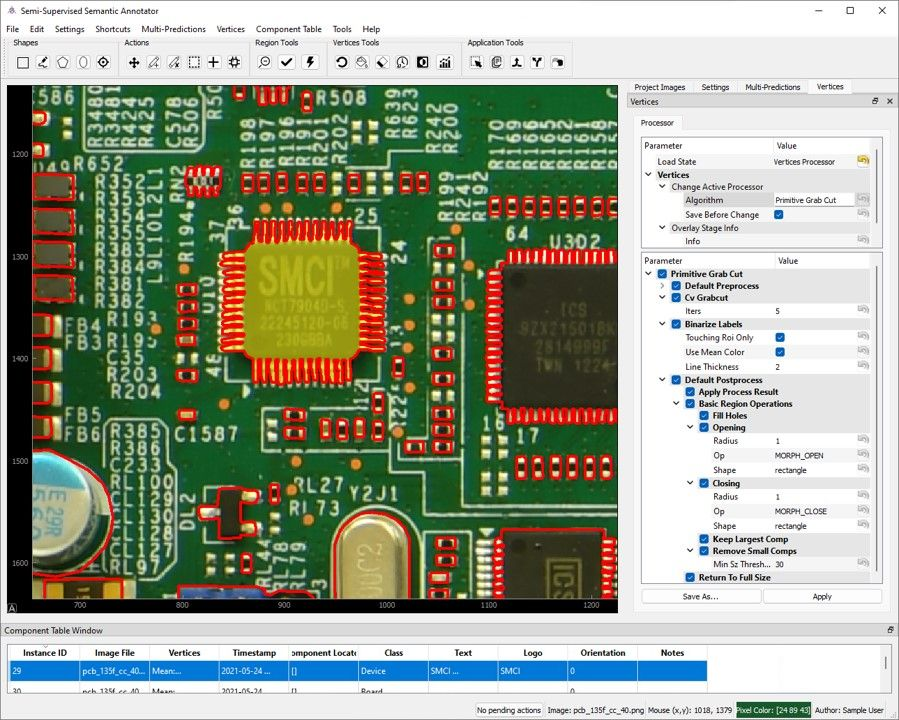
\includegraphics[width=\linewidth]{figures/appOverview}
    \caption{S3A's interface. The main view consists of an image to annotate, a component table of prior annotations, and a toolbar which changes functionality depending on context.}
    \label{fig:appOverview}
\end{figure}
}

\newcommand{\makeCropExportsFig}{%
\begin{figure}[tbp]
    \centering
    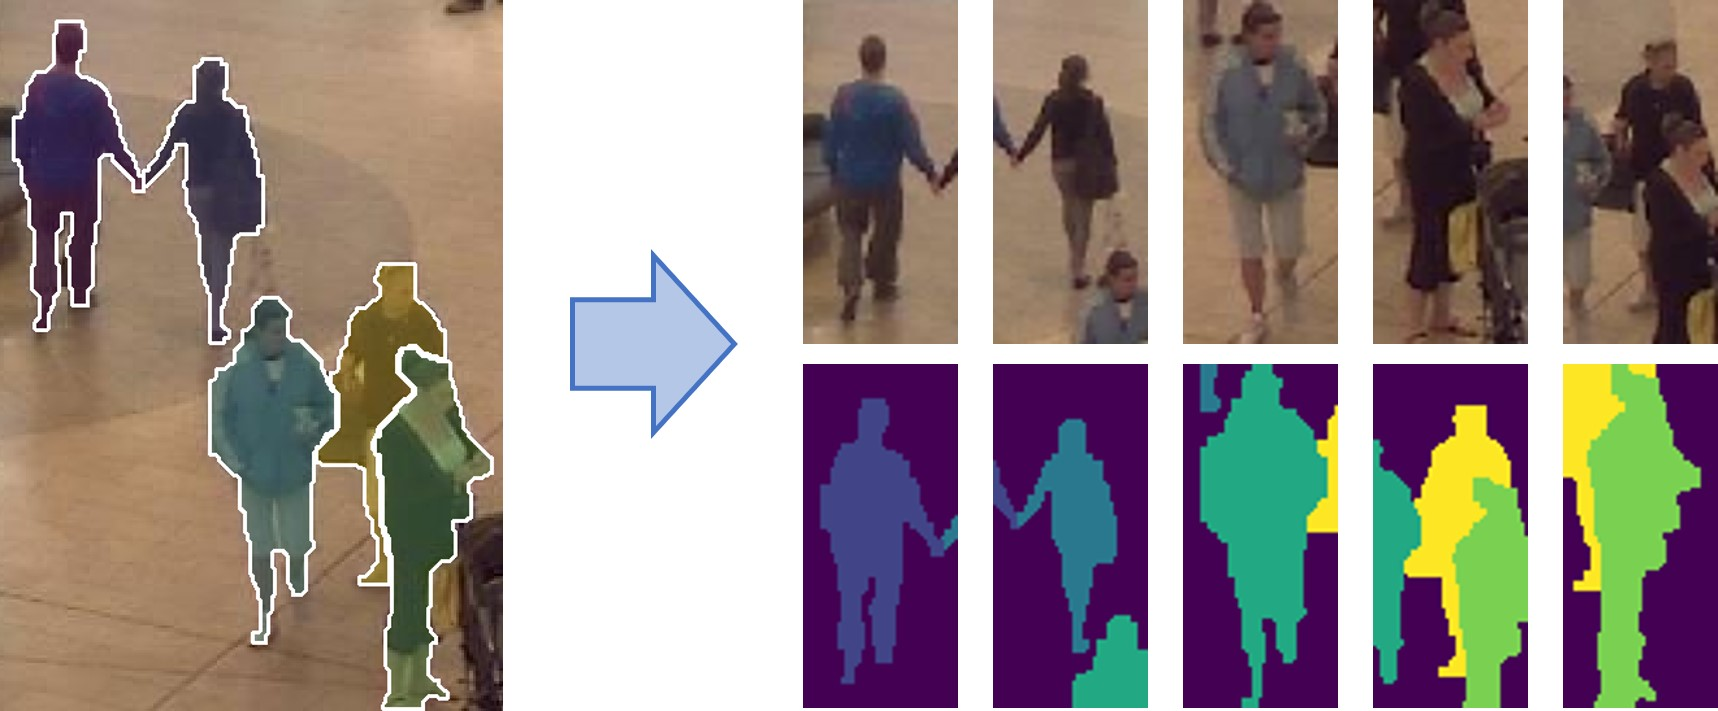
\includegraphics[width=\linewidth]{figures/cropExports}
    \caption{Multiple export formats exist, among which is a utility that crops components out of the image, optionally padding with scene pixels and resizing to ensure all shapes are equal. Each sub-image and mask is saved accordingly, which is useful for training on multiple forms of machine learning models.}
    \label{fig:cropExports}
\end{figure}
}

\newcommand{\makeRegionAnalyticsFig}{%
\begin{figure*}[tbp]
    \centering
    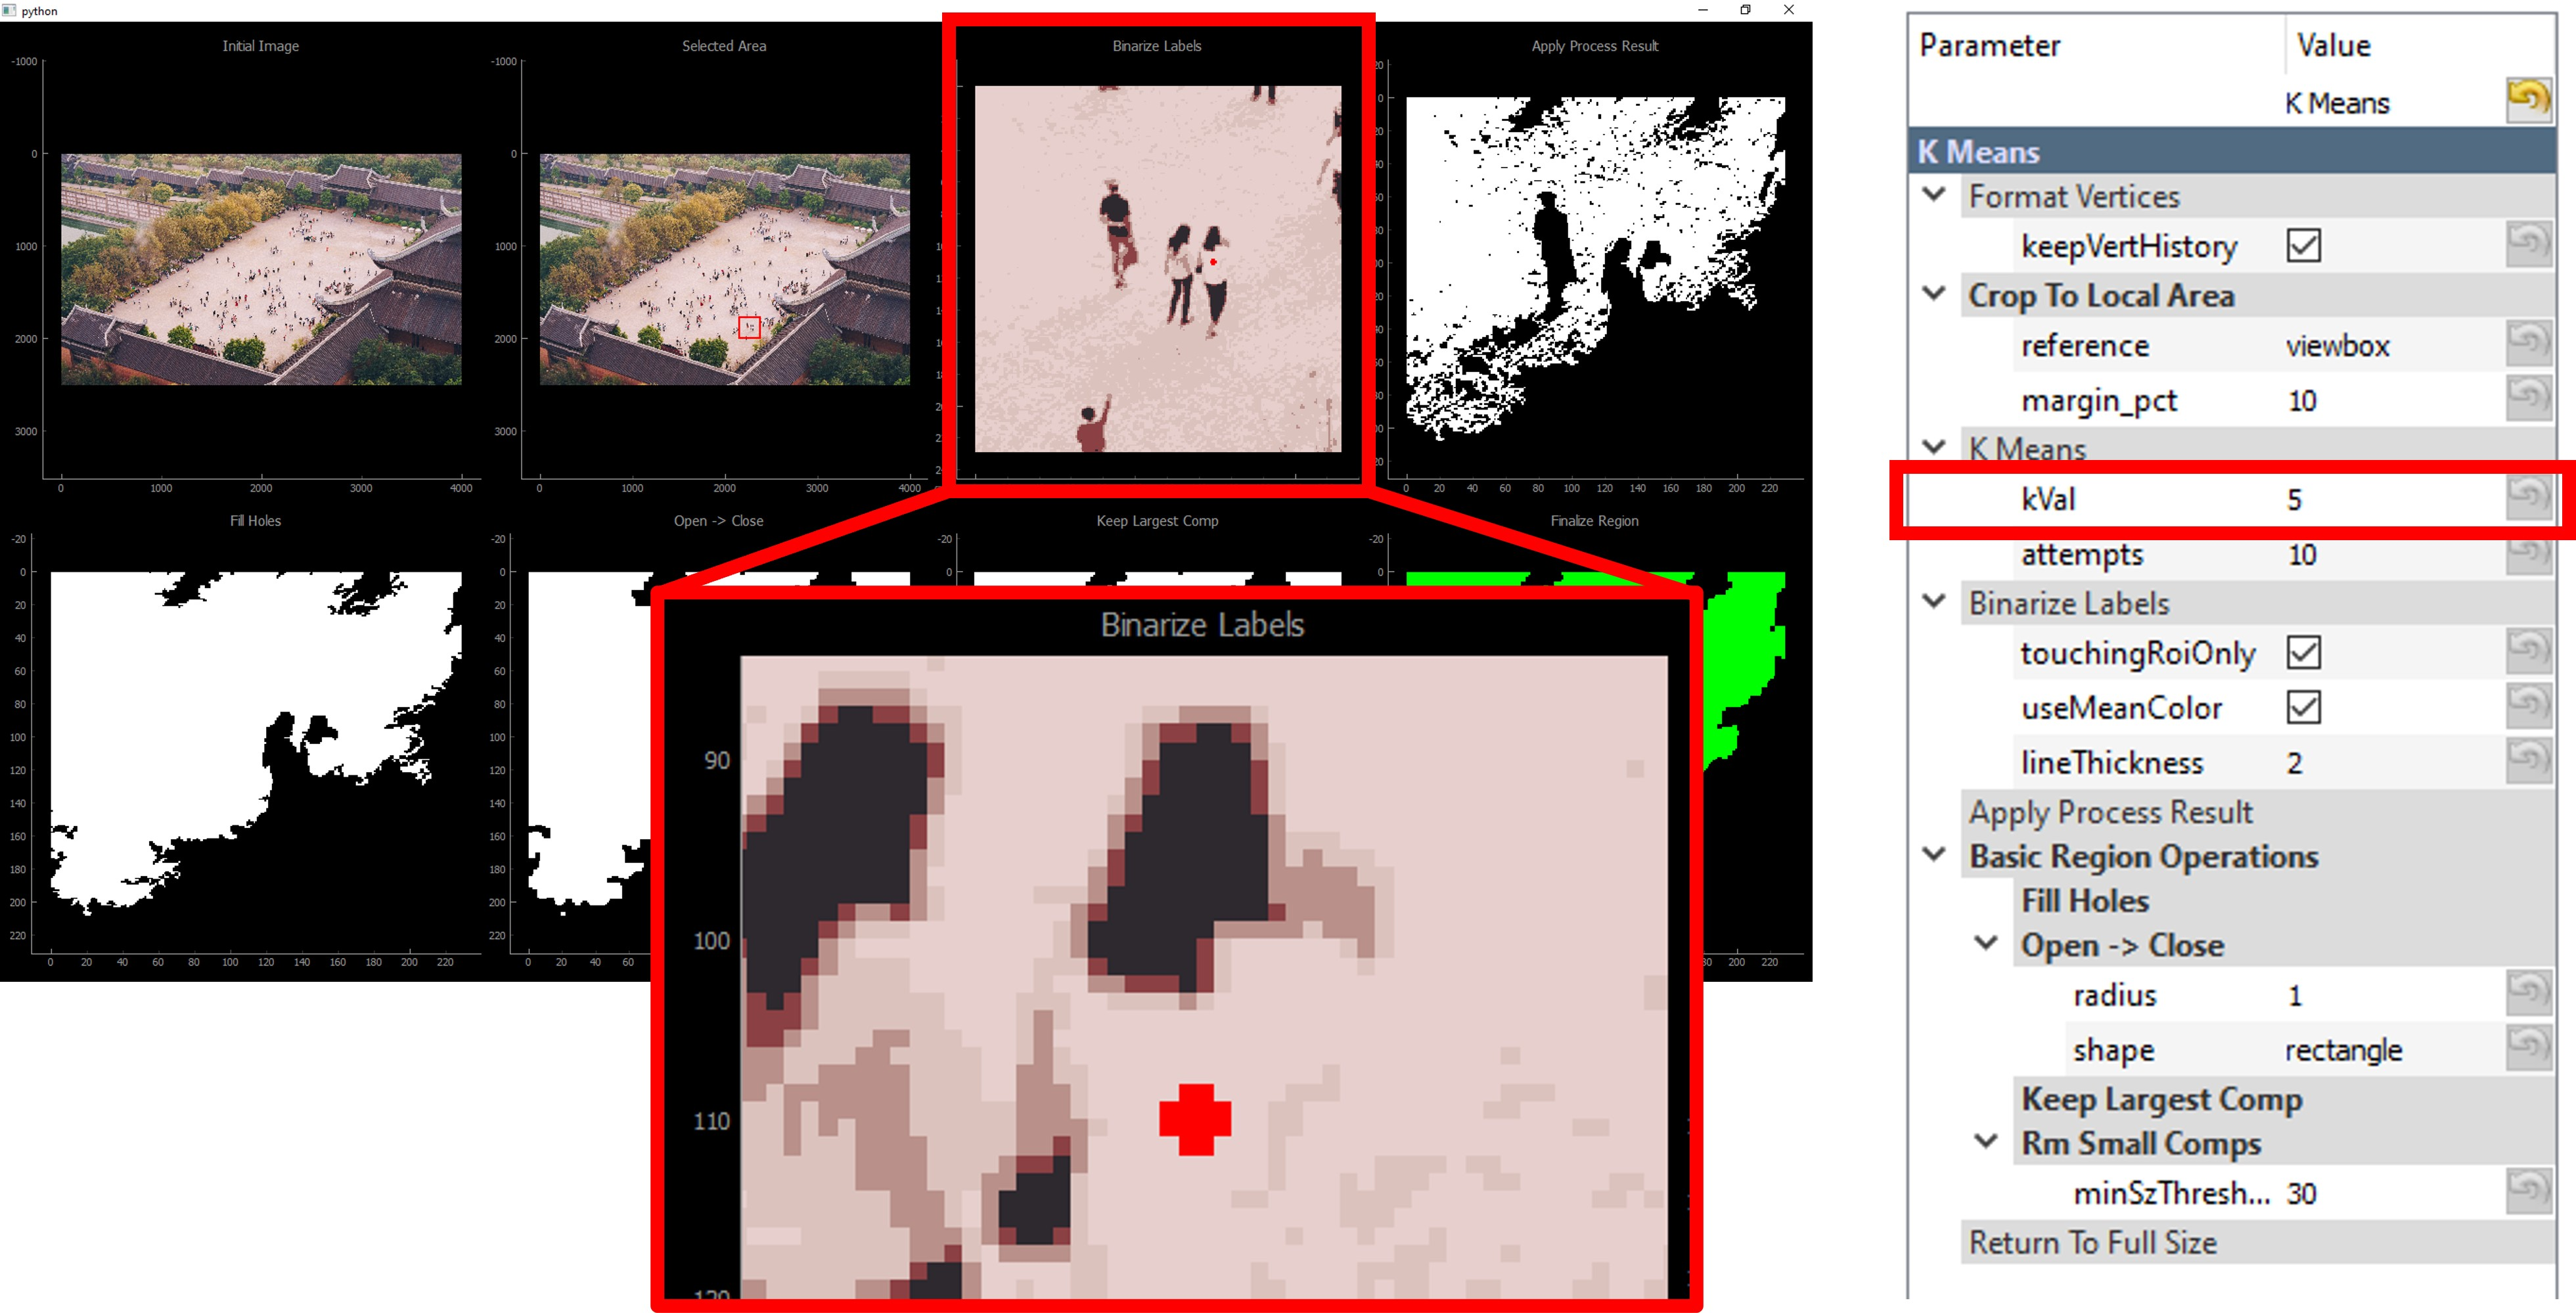
\includegraphics[width=0.7\linewidth]{figures/regionAnalytics}
    \caption{Outputs of each processing stage can be quickly viewed in context after an iteration of annotating. Upon inspecting the results, it is clear the failure point is a low $k$ value during K-means clustering and segmentation. The woman's shirt is not sufficiently distinguishable from the background palette to denote a separate entity. The red dot is an indicator of where the operator clicked during annotation.}
    \label{fig:regionAnalytics}
\end{figure*}
}

\newcommand{\makeRegionEditFig}{
\begin{figure}[tbp]
  \centering
  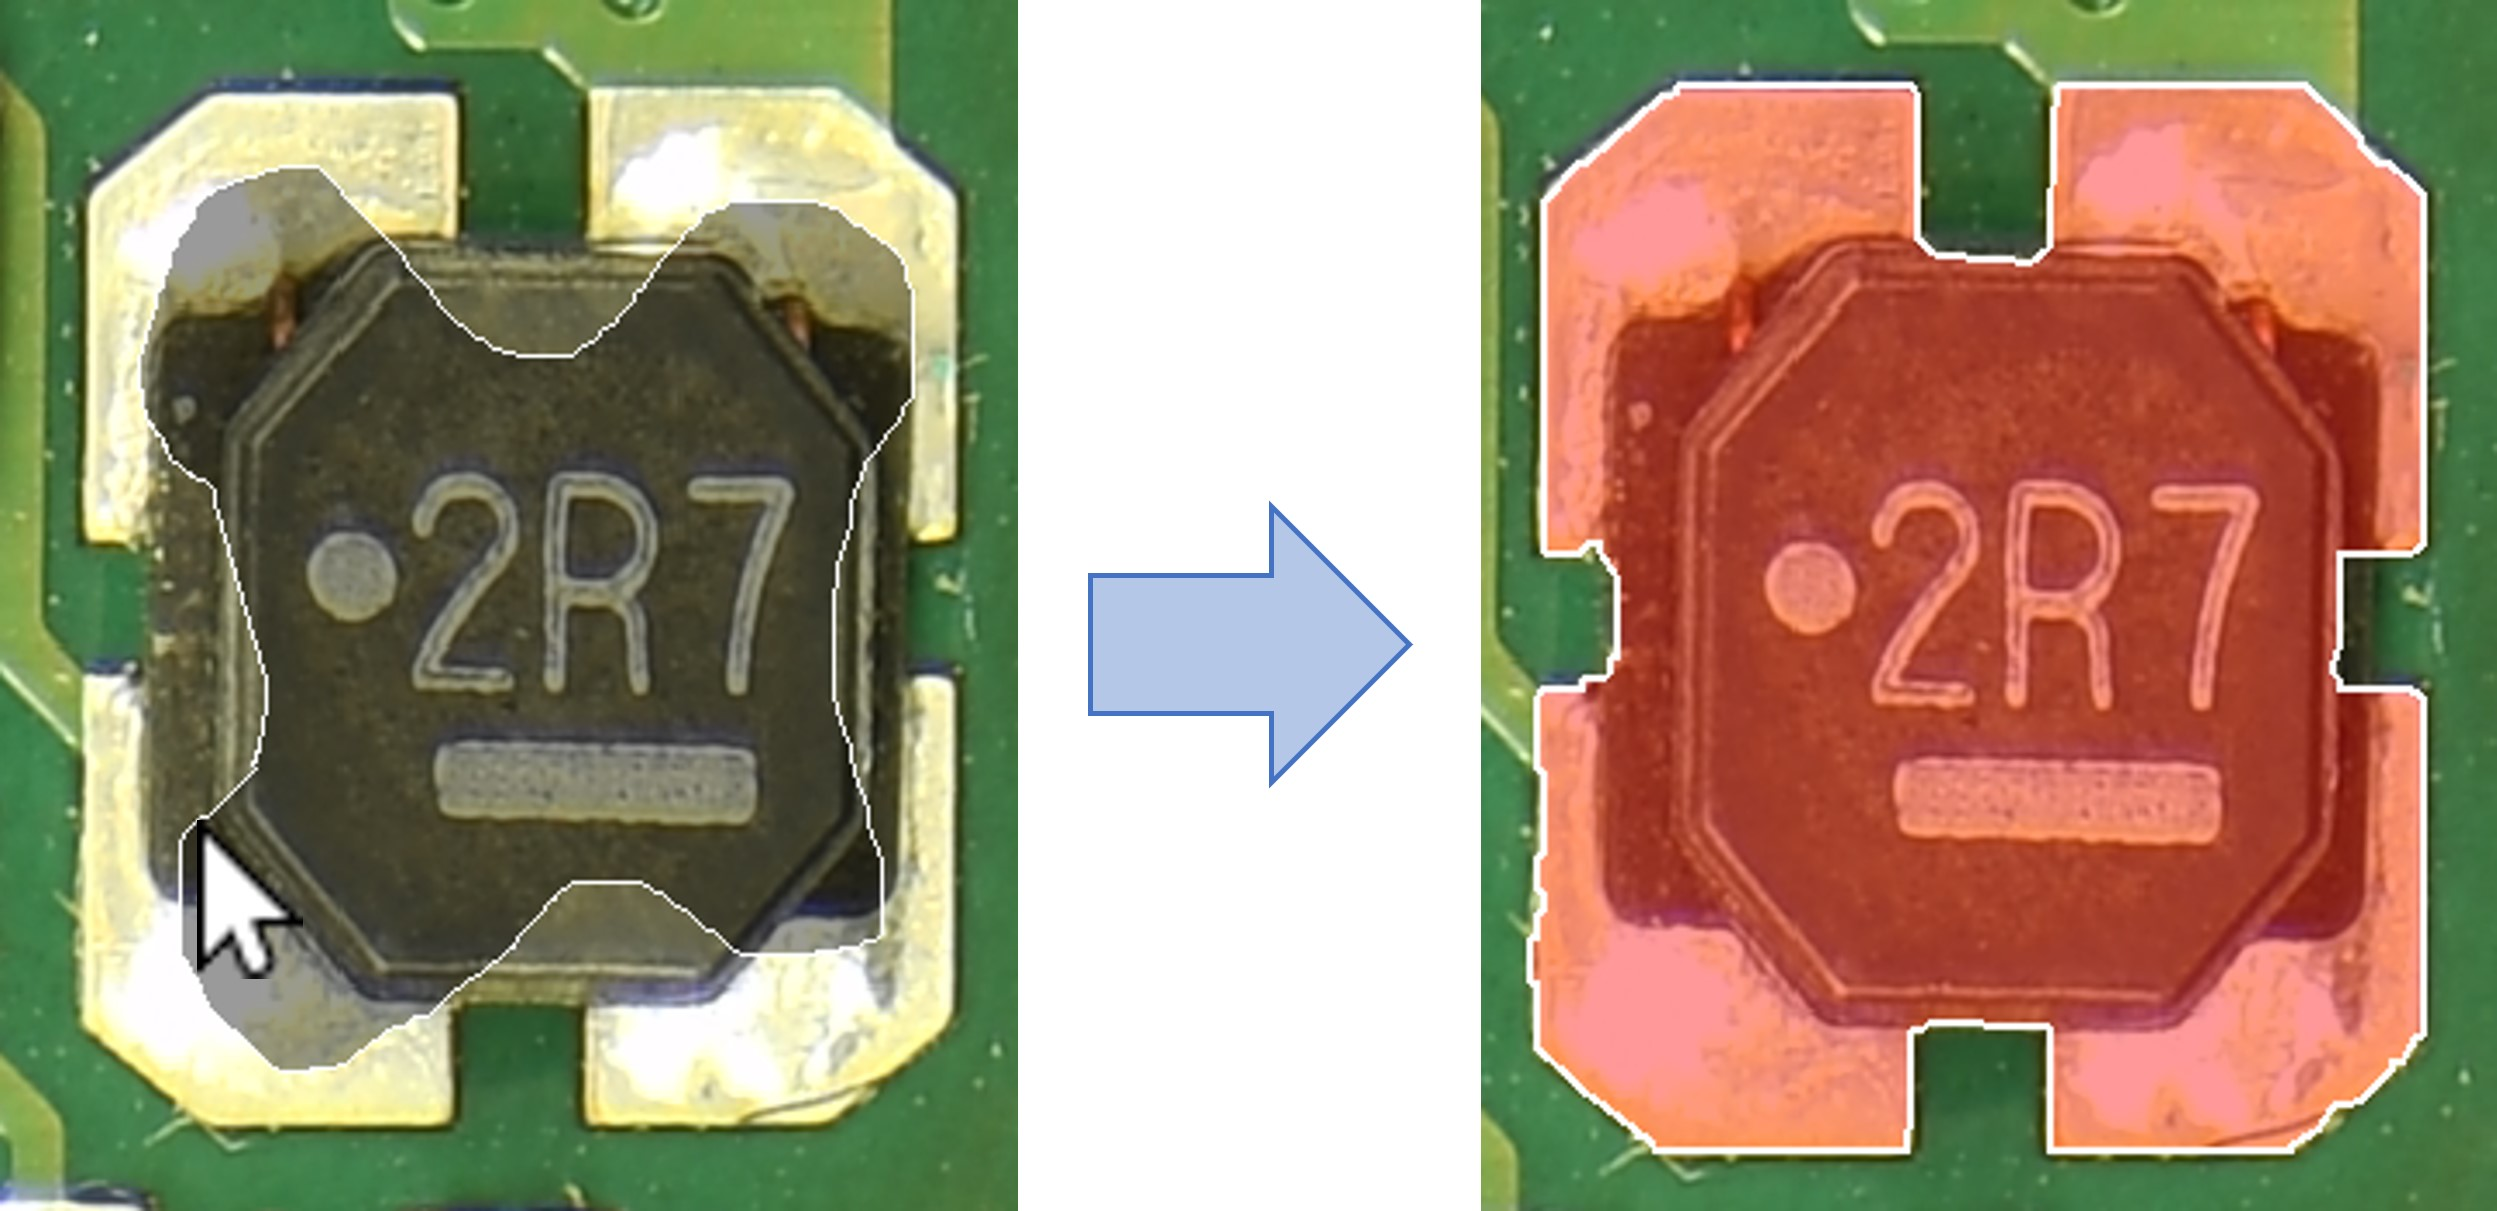
\includegraphics[width=\linewidth]{figures/regionEdit}
  \caption{Regardless of total image size and number of annotations, Python processing is be limited to the ROI or viewbox size for just the selected object based on user preferences. The depiction shows Grab Cut operating on a user-defined initial region within a much larger (8000x6000) image. The resulting region was available in 1.94 seconds on low-grade hardware.}
  \label{fig:regionEdit}
\end{figure}
}

\newcommand{\makeMetadataFig}{
\begin{figure}[tbp]
  \centering
  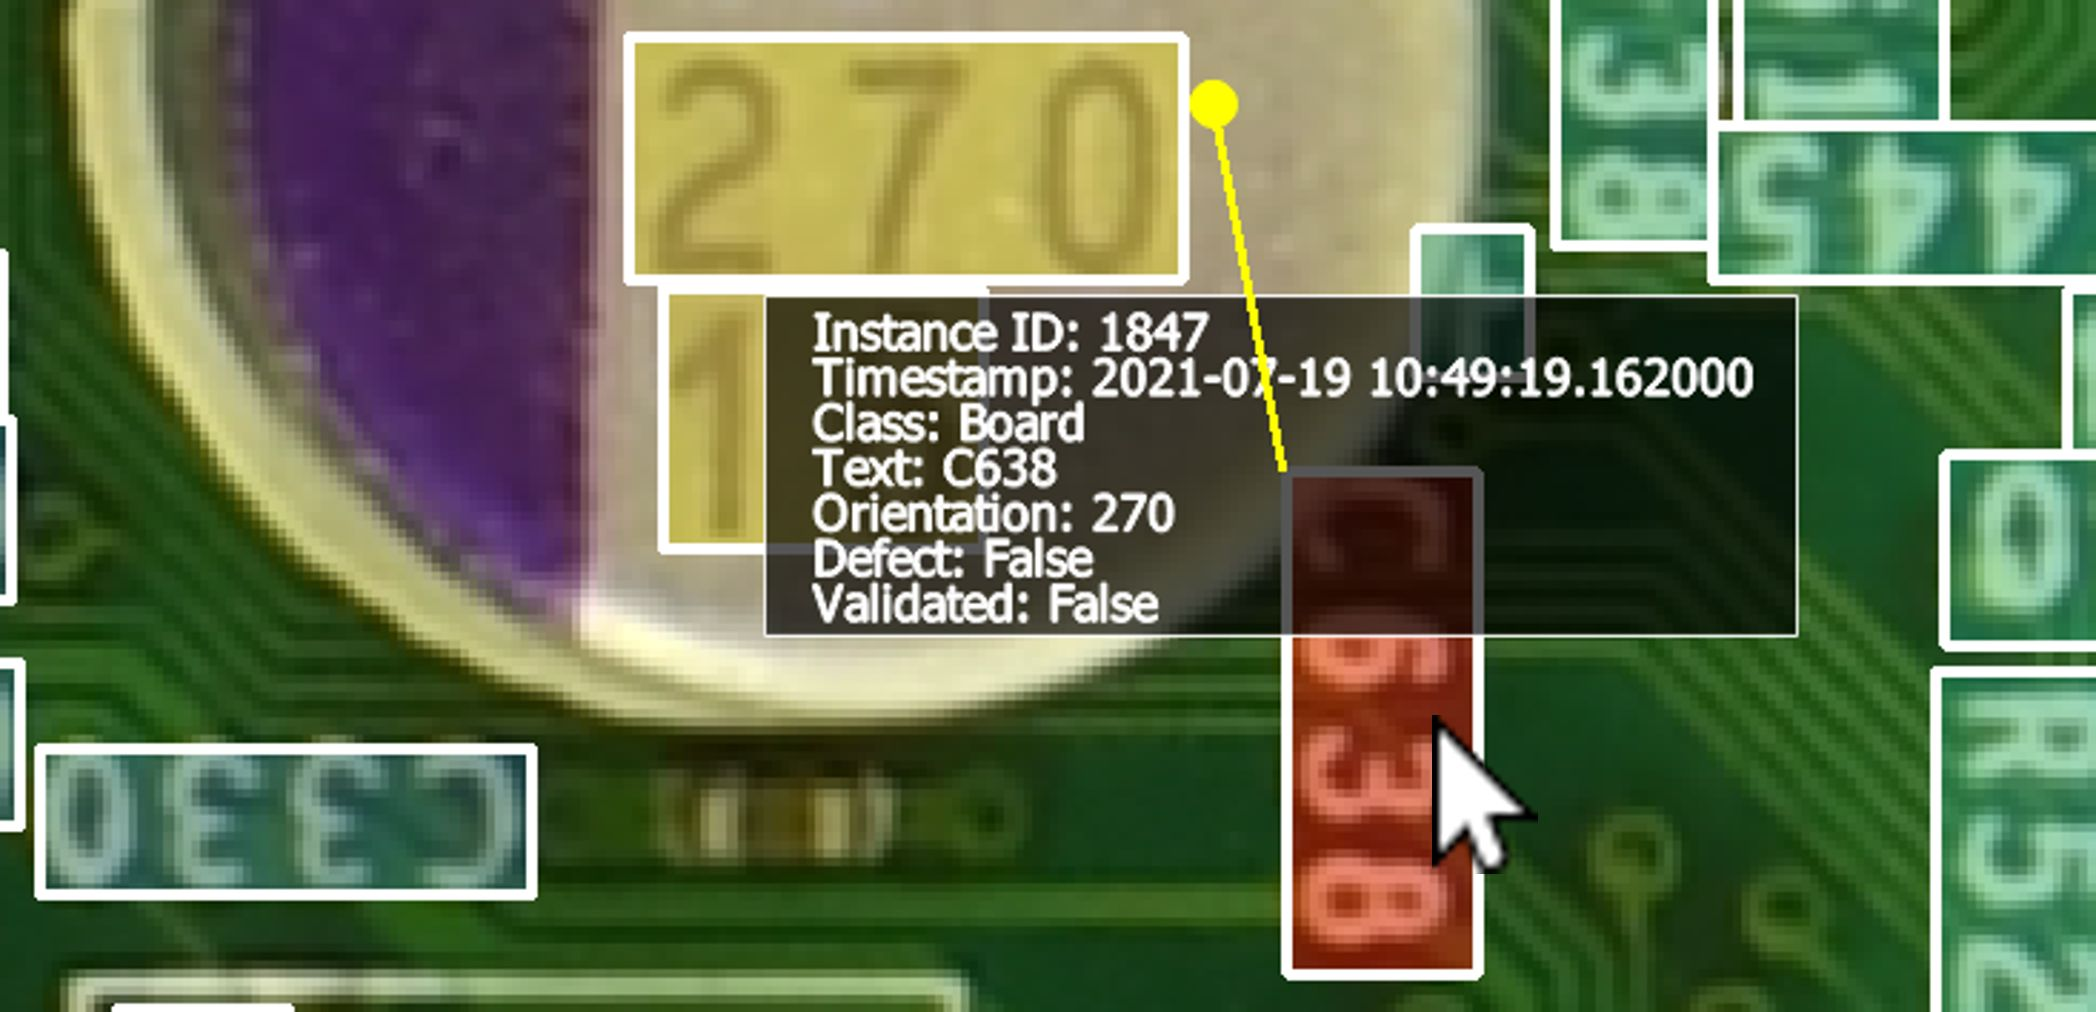
\includegraphics[width=\linewidth]{figures/metadata}
  \caption{Metadata can be collected, validated, and customized with ease. A mix of default properties (strings, numbers, booleans), factories (timestamp, author), and custom plugins (yellow circle representing associated device) are present.}
  \label{fig:metadata}
\end{figure}
}

\newcommand{\makeComplexRegionFig}{
\begin{figure}[tbp]
  \centering
  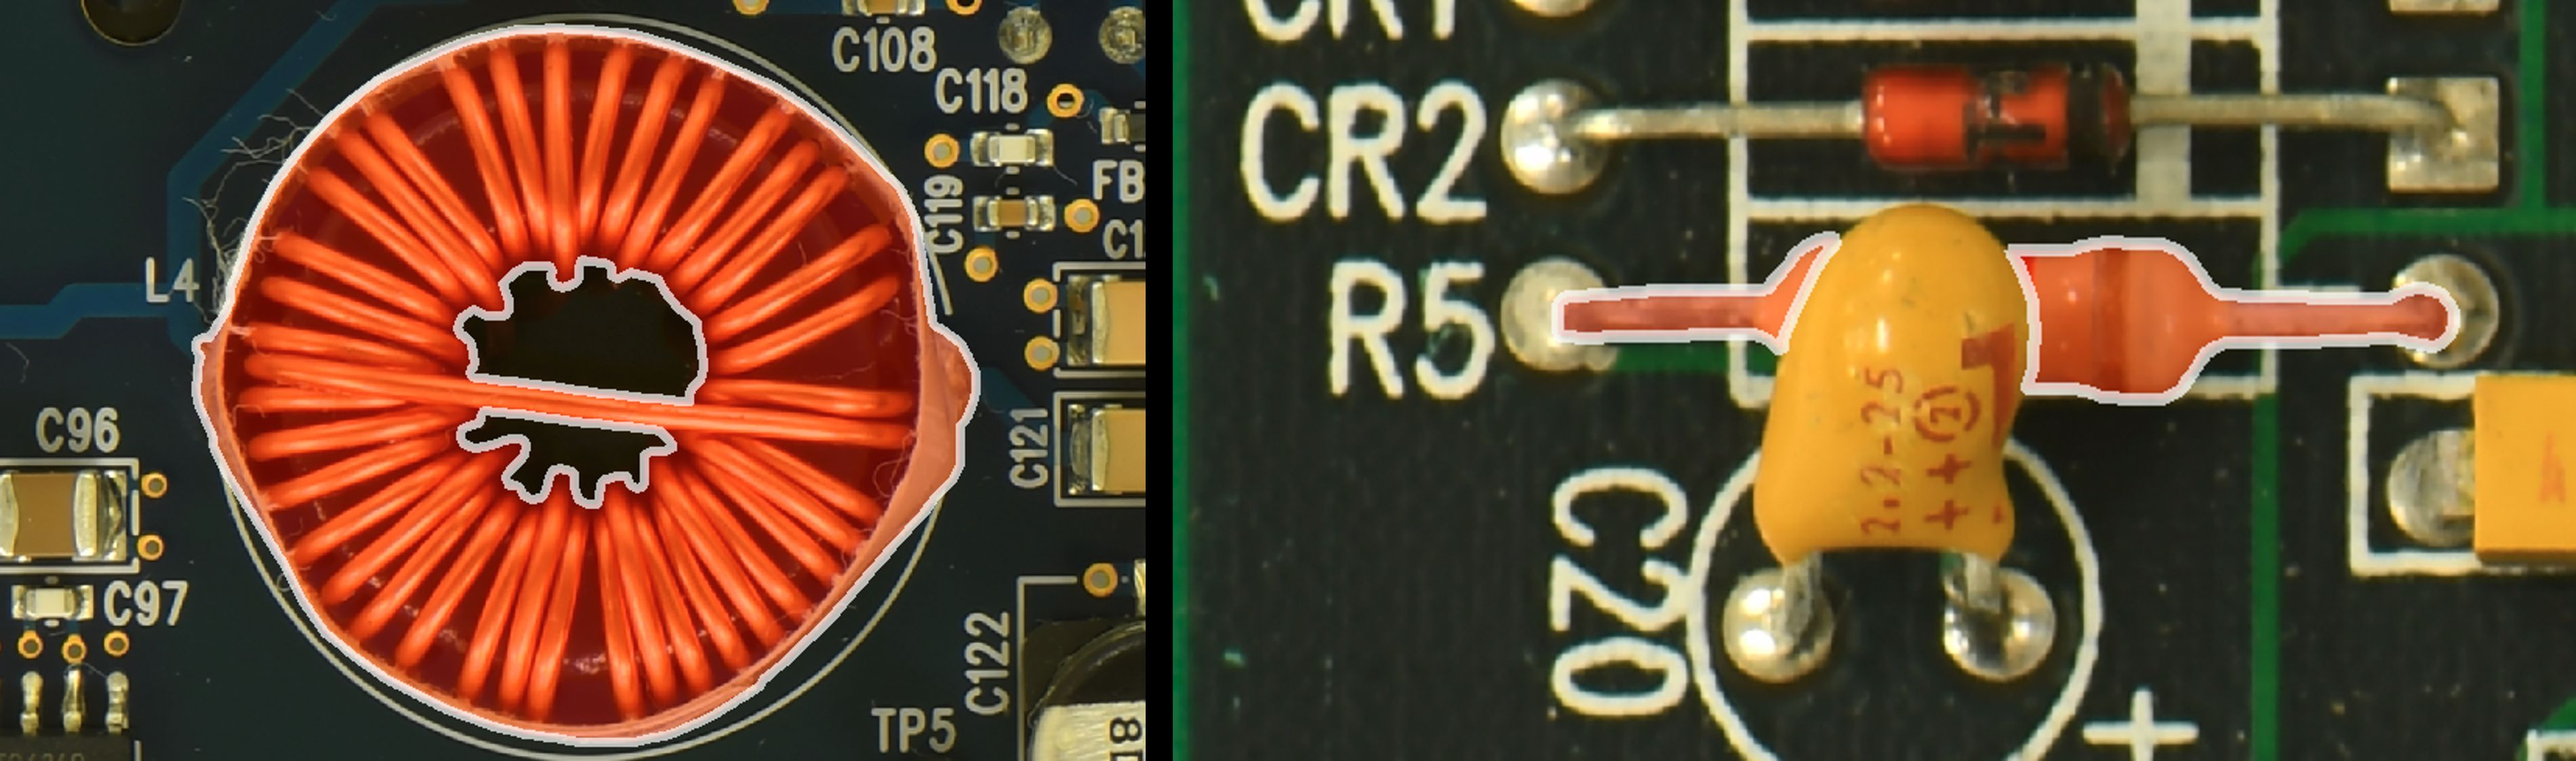
\includegraphics[width=\linewidth]{figures/complexRegion}
  \caption{Annotated objects in S3A can incorporate both holes and distinct regions through a multi-polygon container. Holes are represented as polygons drawn on top of existing foreground, and can be arbitrarily nested (i.e. island foreground is also possible).}
  \label{fig:complexRegion}
\end{figure}
}
